Let's now analyze in some more detail some \patxi{the} results presented in the previous section.

The mean \textbf{Source Compilability} of the projects (47.29\%), although low, is slightly higher than in previous studies on Java projects such as that of Tufano et al (38.13\%). 
This is partly due to having left out 20 projects whose compilability was 0.
But what is more interesting is the differences from project to project, something that was expected, and seen in previous studies on the matter~\cite{tufano2017there,sulir2020large,querel:2021:warning}.

The mean value of the \textbf{Test Compilability\textsubscript{A}} is significantly lower (41.73\%), because Source Compilability is a threshold for this metric.
Moreover, considering only those commits where the source code is compiled, the \textbf{Test Compilability\textsubscript{S}} offers a considerably higher value on average (88\%).
This value is reasonable, since once the main source code was built \patxi{compile?}, it is more likely that the test code can also be built\patxi{compile? Revisar todos los build y built}. 
% What is maybe unexpected, as we will discuss later in Section~\ref{sec:semantics}, is that it is not even higher.
We also note that for this metric, 50\% of the projects offer a value higher than 97\%.\patxi{Therefore, test compilation does not seem a problem in general, and efforts, in any case, should be put in source compilation.}


%In contrast, it seems that the compilability of both source code and tests is significantly lower than for projects collected through the GitHub API. Many4J projects offer a significantly lower mean on all parameters.

The most clear result when analyzing testability of projects is its variability from project to project. 
Figure~\ref{fig:testability-overview} illustrates this, by showing the shape of the distribution of all testability metrics we defined, for all projects.

\begin{figure*}[ht!]
    \centering    
    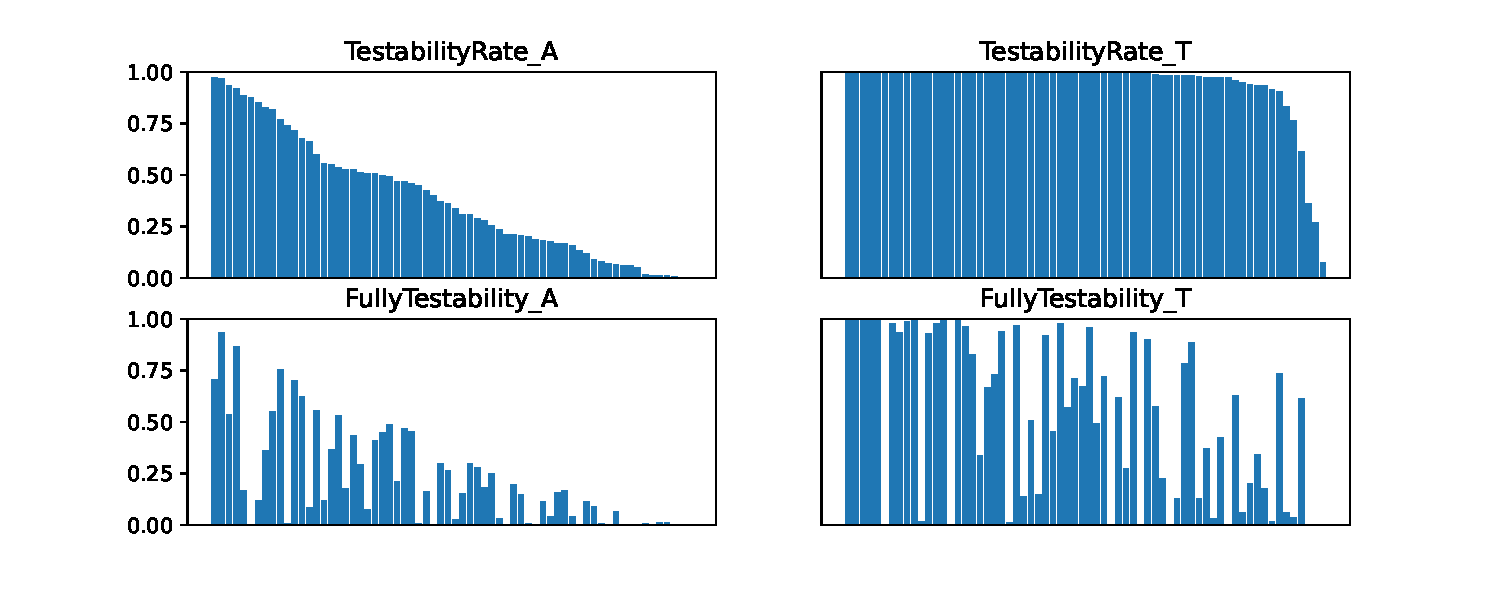
\includegraphics[width=\textwidth]{pages/02-Testability/images/Overview.pdf}
    \caption{Overview of testabilities - Each bar represents a project. Each column\patxi{column? Hay que ver cómo decir esto que se entienda mejor} is ordered by the corresponding Testability Rate (A and T) of each project.}
    \label{fig:testability-overview}
\end{figure*}

Looking at the Testability Rate values, when we focus on those commits where the tests can be built (\textbf{Testability Rate\textsubscript{T}}) we observe an average value of 94.14\%, a high percentage of the project's tests are executed successfully. 
% Again, we see that the \textbf{Testability Rate\textsubscript{T}}, as with other values, varies a lot between projects, with the median of this value being 99.53\%, indicating that in 50\% of the cases almost all the tests pass for test compilable commits.
By calculating the Testability Rate considering all commits (\textbf{Testability Rate\textsubscript{A}}), this value gives an overview of the testability of the project and how Source Compilability impacts running tests on past commits.

Focusing on \textbf{Fully Testability\textsubscript{T}}, we could expect it would be usually high: developers should write code that does not break \textit{all} the tests. 
Fact is that in more than half of the commits that were test-compilable some tests fail when they are run. 
This result, which may seem surprising, deserves as well more discussion that we will provide in Section~\ref{sec:low-testability}.\patxi{¿Por qué no aquí si estamos en la sección de análisis?}

\textbf{Fully Testability\textsubscript{A}} gives quite interesting information: the fraction of commits that are testable, with respect to the total number of commits. 
When compilability is low, this fraction is necessarily low, just meaning that commits are not testable because they are not source- or test-compilable. 
When compilability is high, \textit{Fully Testability\textsubscript{A}} really shows differences.\patxi{¿Qué diferencias¿Entre proyectos? -> among projects} 

With the data presented up to here, we can already answer RQ\textsubscript{1}, RQ\textsubscript{2} and RQ\textsubscript{3}\patxi{Ojo, la numeración de las RQs ha cambiado: 2.1, 2.2, 2.3, y en los siguientes párrafos igual}:

\vspace{0.5cm}
\fbox{\begin{minipage}{\textwidth}
\textbf{\textbf{RQ\textsubscript{1}}: ``\RQI''}
We found 93,925 test-compilable commits out of 103,097 source-compilable commits.
When calculating \textit{Test Compilability} using all the commits of the project we obtain an average value of 41.73\%, while if we compute only the commits in which we can compile the source code, the average value increases significantly (88.2\%).\patxi{Hay que aportar algo más aquí que sólo los datos. ¿Qué implica esto?: We can conclude that when the source code compiles, the test code compile, therefore, in general, test compilation is not an issue.}
\end{minipage}}

\vspace{0.5cm}
\fbox{\begin{minipage}{\textwidth}
\textbf{\textbf{RQ\textsubscript{2}}: ``\RQII''}
We found 40,540 fully-testable commits out of 93,925 test-compilable commits. 
When calculating \textit{Fully Testability} using all the commits of the project we obtain an average value of 22.12\%, while if we compute only the commits in which we can compile the tests, the average value increases significantly (52.53\%).\patxi{This is quite surprising, as one would expect that all tests should pass before a commit is accepted (after all, this is what CI is for). The results that we show here indicates that this is not always the case. We discuss it further in the next section.}
\end{minipage}}

\vspace{0.5cm}
\fbox{\begin{minipage}{\textwidth}
\textbf{\textbf{RQ\textsubscript{3}}: ``\RQIII''}
When calculating \textit{Testability Rate} using all the commits of the project we obtain an average value of 38.63\%, while if we compute only the commits in which we can compile the tests, the average value increases significantly (94.14\%).\patxi{This is in line with our expectations: in general when the tests compile, they succeed.}
\end{minipage}}
    
